%************************************************
\chapter{The Mind Monitor Application}
\label{chapter:the_mind_monitor_application}
%************************************************

In order to control the SALS model of mind, a mind monitoring
application called \emph{MindMon} has been implemented.  MindMon is
based on abstract physical world and reflective thinking components
that allow reflective thinking layers to be interchanged with
different $\text{reflective}^0$ physical layers.  In this dissertation
I focus on a block building domain in order to demonstrate
second-order reflective learning to plan, but other more complex
physical domains have also been developed within SALS such as the
IsisWorld physical simulator described by \cite{smith:2010}, where
MindMon allows attaching multiple reflective thinking models to a
shared $\text{reflective}^0$ physical layer, a type of simulation that
assumes a more complex subjective philosophy of mind that is not
assumed in the non-subjective model described in
{\mbox{\autoref{part:the_model}}} of this thesis.
{\mbox{\autoref{figure:implemented_mindmon}}} shows the MindMon
application.
\begin{figure}
\hspace*{-1cm}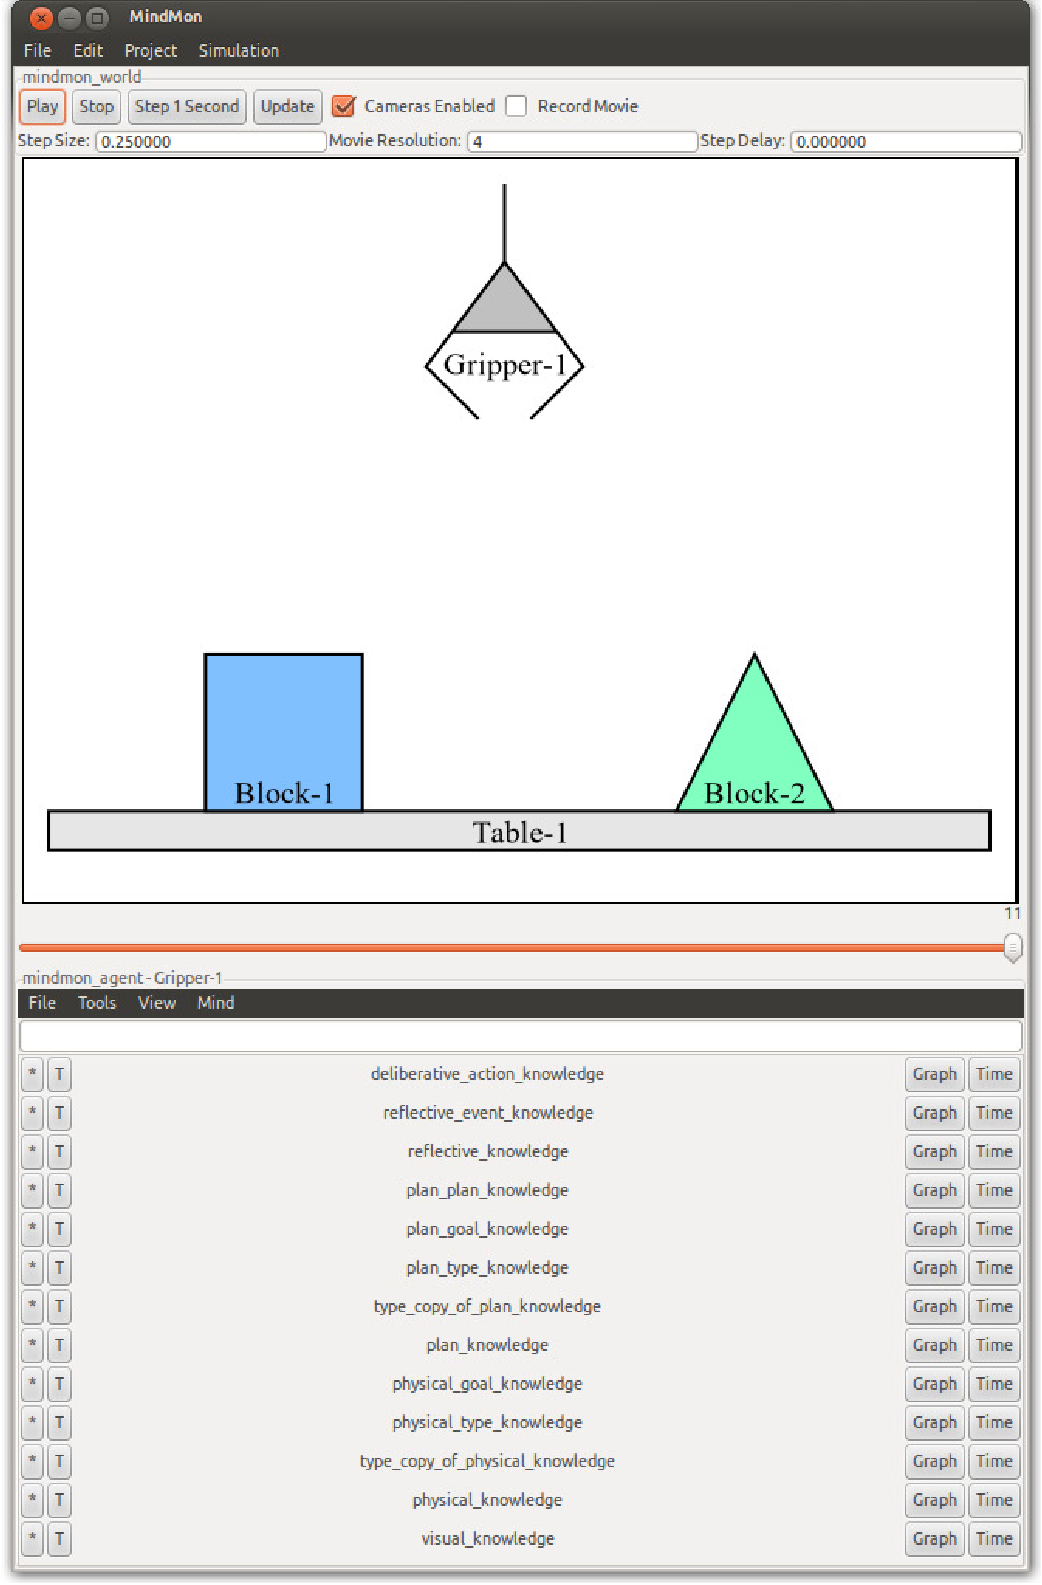
\includegraphics[width=13cm]{gfx/implemented_mindmon}
\caption[The mind monitoring application, MindMon.]{The mind
  monitoring application, MindMon, shown here with the simple block
  building domain and the reflective thinking layers described in this
  dissertation.}
\label{figure:implemented_mindmon}
\end{figure}

\section{The Physical Knowledge-Base}

The block building domain is a simulation based on two-dimensional
ridid-body physical laws, including floating point numerical
representations for object positions, velocities and accellerations.
These numerical representations and the processes that manipulate them
are part of the $\text{reflective}^0$ physical layer of the model, but
in order to focus the efficiency of the procedural reflection, a much
simpler relational graph representation has been specifically
represented in semantic frame-based objects in a semantic
knowledge-base, referred to as the \emph{physical knowledge-base}.
The physical knowledge-base includes objects with shapes, colors, and
multiple prepositional spatial relationships.
{\mbox{\autoref{figure:implemented_physical_knowledge}}} shows the
physical knowledge-base.
\begin{sidewaysfigure}
\begin{center}
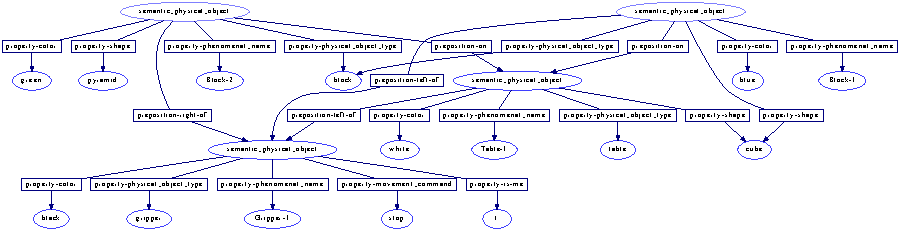
\includegraphics[width=24cm]{gfx/implemented_physical_knowledge}
\end{center}
\hspace{4cm}\parbox{15cm}{\caption[The physical knowledge-base.]{The
    physical
    knowledge-base.}\label{figure:implemented_physical_knowledge}}
\end{sidewaysfigure}

\section{Semantic Event Interval-Tree Knowledge-Base}

Semantic event interval-tree knowledge-bases are used for organizing
all of the remembered history of symbolic perceptions, symbolic
resource activations, as well as symbolic goal activation events.  The
version-space hypothesis concept learning algorithm
{\mbox{\cite[]{mitchell:1997}}} references these interval-tree
structures, which also contain other relevant information, such as
what compiled resource causes the activation of another resource.  In
this way, all interactions between built-in and learned reactive
resources are recorded.
{\mbox{\autoref{figure:implemented_reflective_event_knowledge_base}}}
shows an example overview of a large semantic event interval-tree
knowledge-base, while
{\mbox{\autoref{figure:implemented_semantic_event_knowledge_base}}}
shows a readable small part of an example semantic event interval-tree
knowledge-base.
\begin{figure}
\begin{center}
\hspace*{-2cm}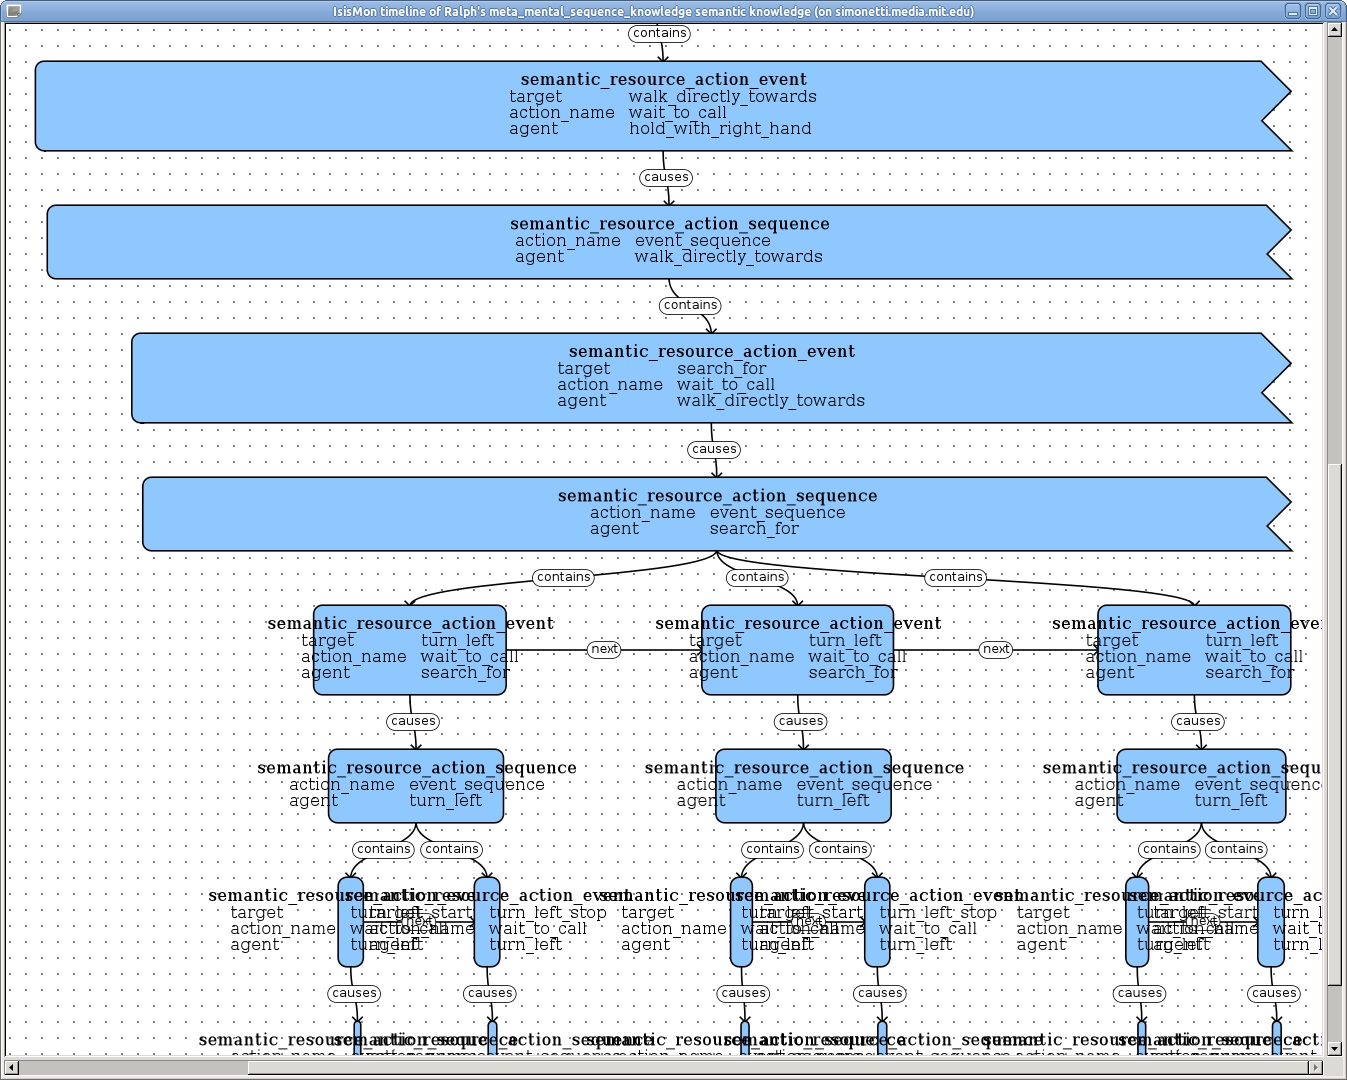
\includegraphics[width=13cm]{gfx/implemented_reflective_event_knowledge_base}
\end{center}
\caption[An example overview of a large semantic event interval-tree
  knowledge-base.]{An example overview of a large semantic event
  interval-tree knowledge-base.  See
  {\mbox{\autoref{figure:implemented_semantic_event_knowledge_base}}}
  for a readable view.}
\label{figure:implemented_reflective_event_knowledge_base}
\end{figure}
\begin{figure}
\begin{center}
\hspace*{-3cm}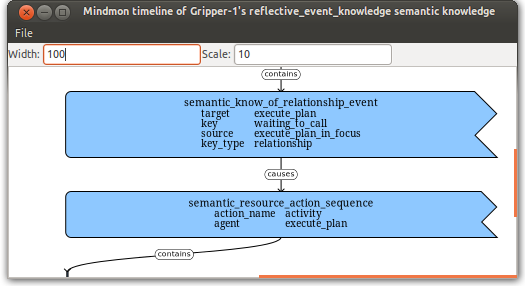
\includegraphics[width=15cm]{gfx/implemented_semantic_event_knowledge_base}
\end{center}
\caption[A close-up view of the semantic event interval-tree
  knowledge-base.]{A close-up view of the semantic event interval-tree
  knowledge-base.  Note the ``contains'' and ``causes'' extra semantic
  relationships between resource activation events.  Event sequences
  for one compiled resource contain sequential plan steps, while
  activations of parallel executing resources are shown as cause
  relationships.  See
  {\mbox{\autoref{figure:implemented_reflective_event_knowledge_base}}}
  for a more global perspective.}
\label{figure:implemented_semantic_event_knowledge_base}
\end{figure}

\section{First-order Resource Activator}

Every resource in SALS is available for user-interaction by using the
activators and monitors of the interchangeable reflective thinking
objects of the Mind Monitor application.  The SALS reflective thinking
layers have been tested with a number of interchangeable
$\text{reflective}^0$ physical layers.
{\mbox{\autoref{figure:implemented_first_order_resource_activator}}}
shows the simplest of these interchangeable $\text{reflective}^0$
physical layers, the built-in reactive symbolic resources of the block
building domain.
\begin{figure}
\begin{center}
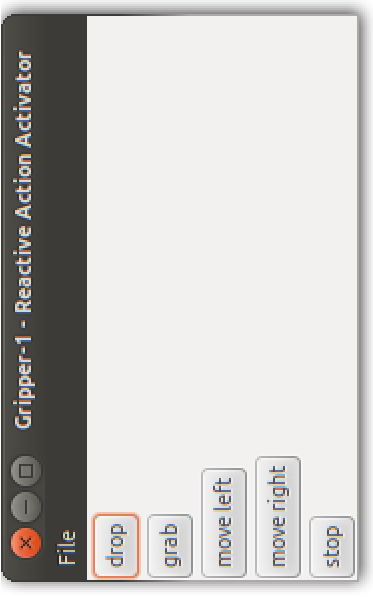
\includegraphics[width=8cm]{gfx/implemented_first_order_resource_activator}
\end{center}
\caption[The first-order resource activator.]{The first-order resource
  activator.}
\label{figure:implemented_first_order_resource_activator}
\end{figure}
%{\mbox{\autoref{figure:implemented_isisworld_first_order_resource_activator}}}
%shows the IsisWorld first-order resource activator.
%\begin{figure}
%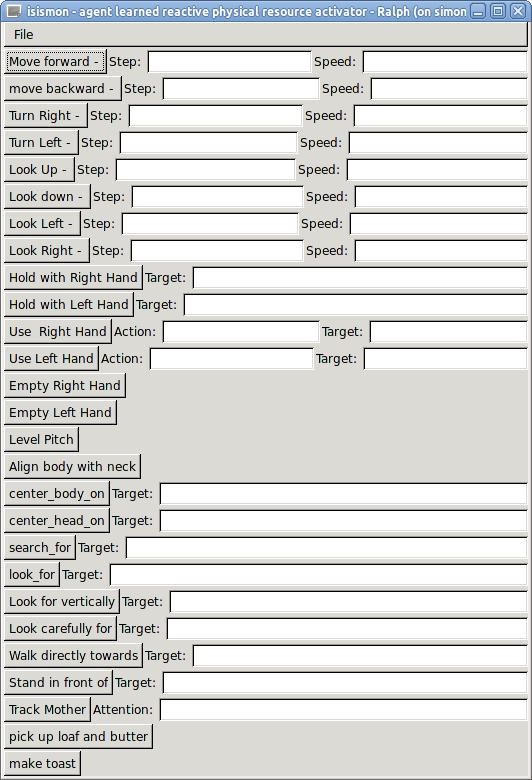
\includegraphics[width=11cm]{gfx/implemented_isisworld_first_order_resource_activator}
%\caption[The implemented IsisWorld first-order resource
%  activator.]{The IsisWorld first-order resource
%  activator.  These resources were by Jing Jian.}
%\label{figure:implemented_isisworld_first_order_resource_activator}
%\end{figure}

\section{First-order Planning Machine Knowledge}

{\mbox{\autoref{implemented_planning_machine_knowledge_detailed}}}
shows the first-order planning machine knowledge-base, while
{\mbox{\autoref{figure:implemented_planning_machine_knowledge}}} shows
a readable zoomed in view.
\begin{sidewaysfigure}
\begin{center}
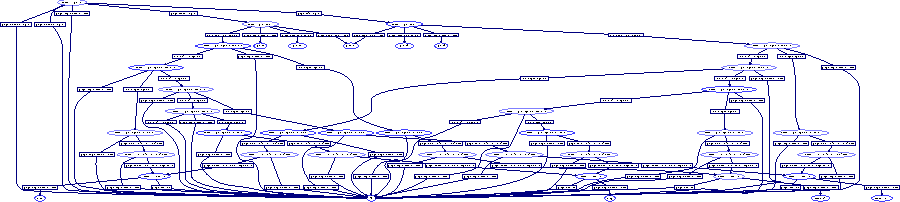
\includegraphics[width=24cm]{gfx/implemented_planning_machine_knowledge_detailed}
\end{center}
\hspace{4cm}\parbox{15cm}{\caption[The physical knowledge-base.]{The
    physical
    knowledge-base.}\label{figure:implemented_planning_machine_knowledge_detailed}}
\end{sidewaysfigure}
\begin{figure}
\begin{center}
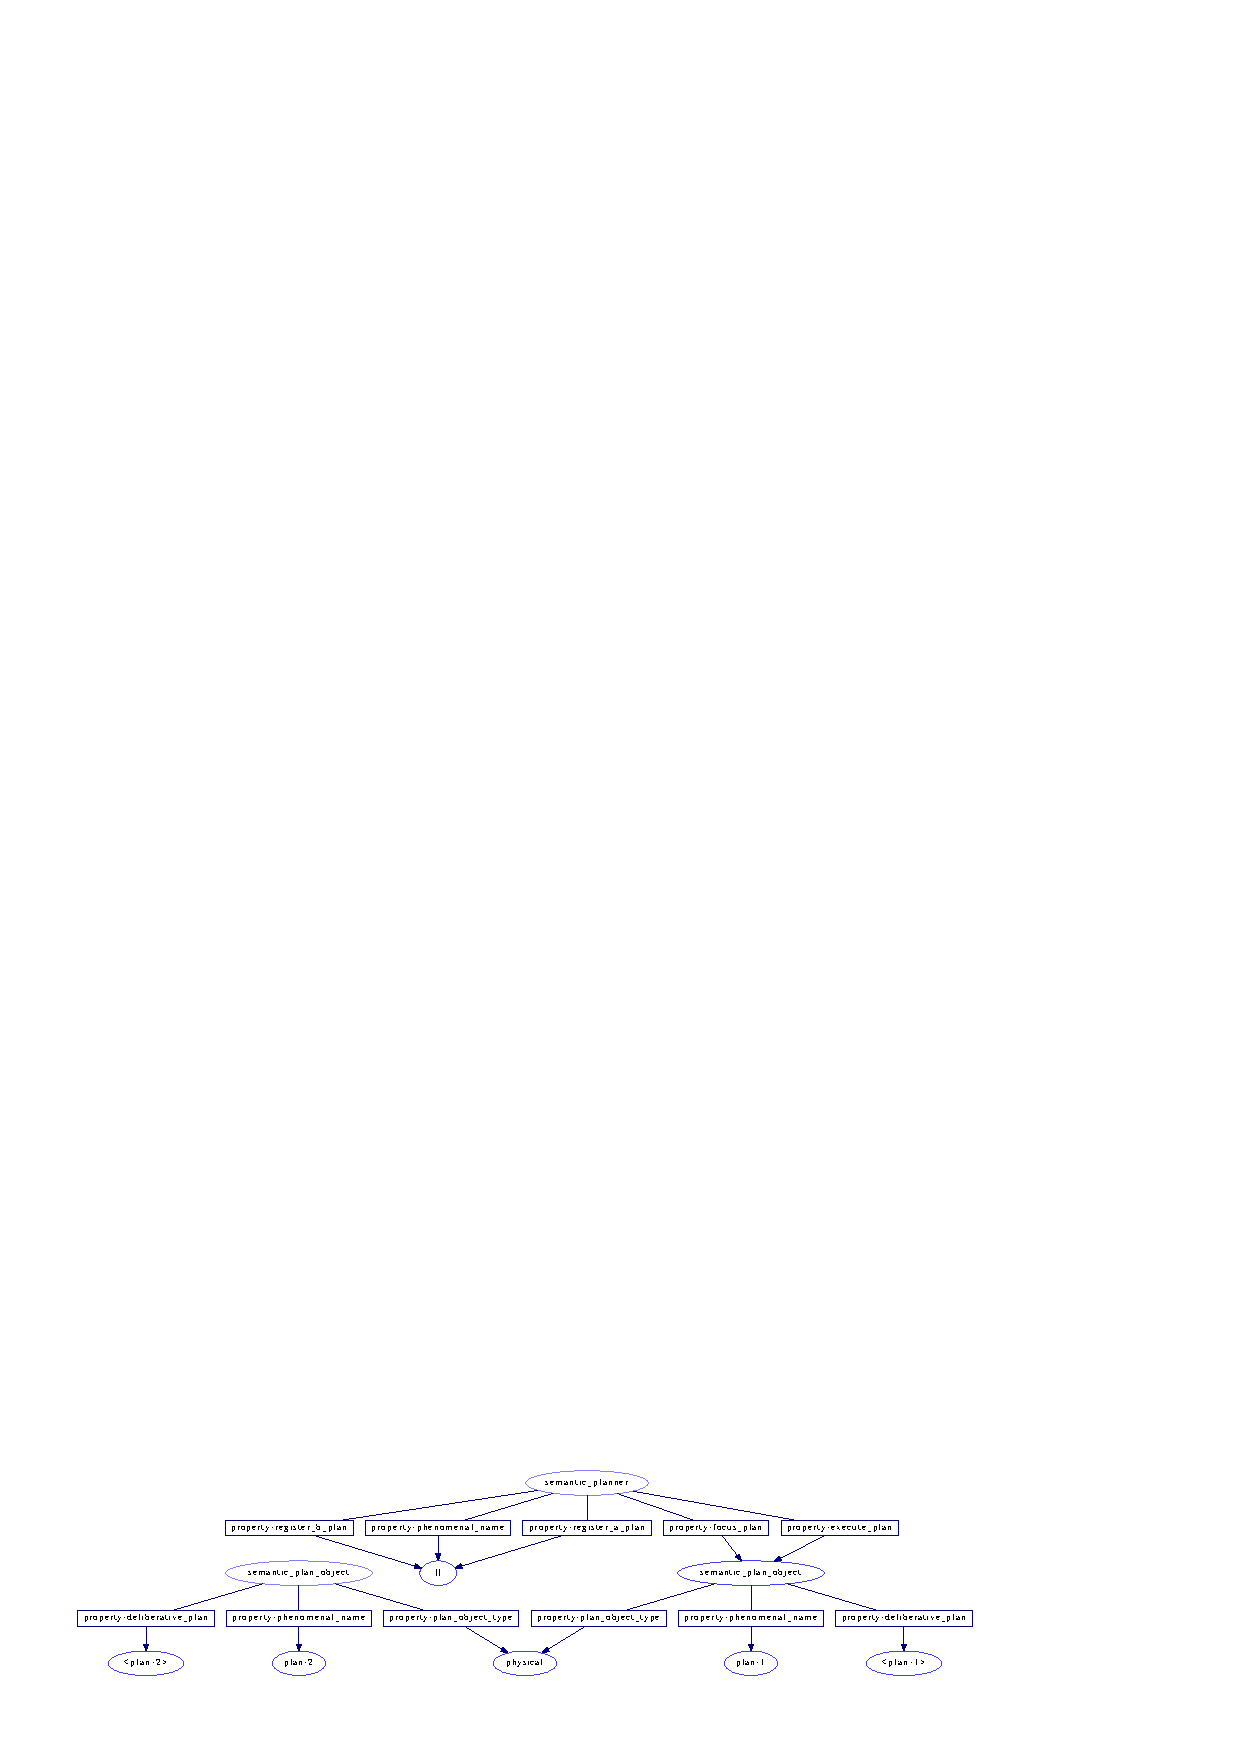
\includegraphics[width=14cm]{gfx/implemented_planning_machine_knowledge}
\end{center}
\caption[The first-order planning machine knowledge-base.]{The
  first-order planning machine knowledge-base.}
\label{figure:implemented_first_order_planning_machine_knowledge}
\end{figure}

\section{First-order Plan Activator}

{\mbox{\autoref{figure:implemented_first_order_plan_activator}}} shows
the first-order plan activator.
\begin{figure}
\begin{center}
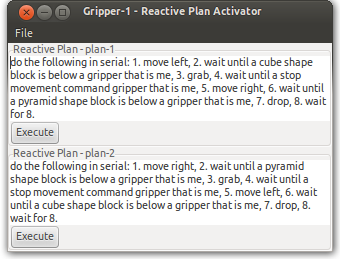
\includegraphics[width=10cm]{gfx/implemented_first_order_plan_activator}
\end{center}
\caption[The first-order plan activator.]{The first-order plan
  activator.}
\label{figure:implemented_first_order_plan_activator}
\end{figure}

\section{Second-order Resource Activator}

{\mbox{\autoref{figure:implemented_second_order_resource_activator}}}
shows the second-order resource activator.
\begin{figure}
\begin{center}
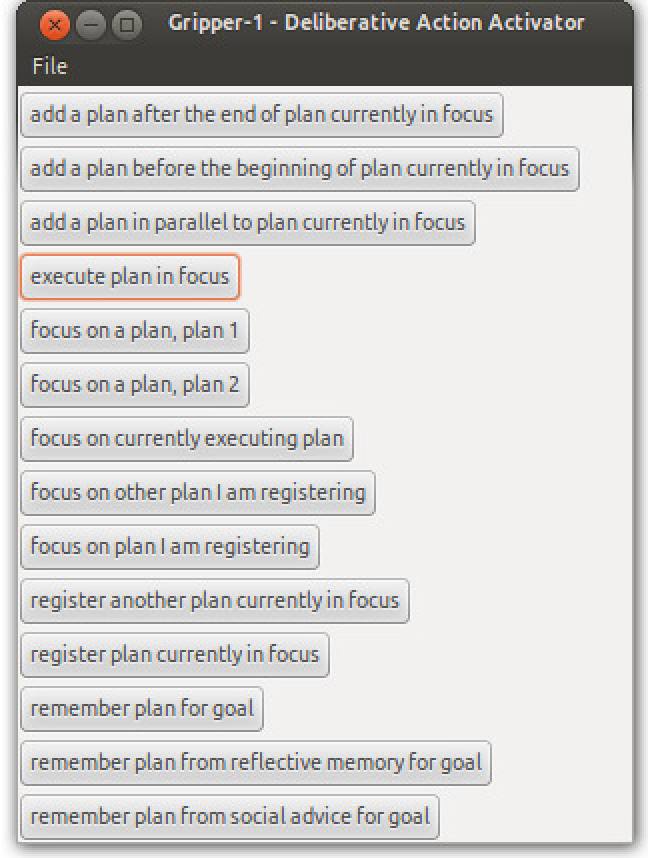
\includegraphics[width=10cm]{gfx/implemented_second_order_resource_activator}
\end{center}
\caption[The second-order resource activator.]{The second-order
  resource activator.}
\label{figure:implemented_second_order_resource_activator}
\end{figure}

